\documentclass[12pt, a4paper]{extarticle}
\usepackage[colorlinks=true,
linkcolor=black,
anchorcolor=black,
citecolor =blue,
filecolor = cyan,
menucolor =red,
urlcolor =magenta]{hyperref}

\usepackage{graphicx}
\usepackage{pagecolor,lipsum}% http://ctan.org/pkg/{pagecolor,lipsum}
\definecolor{anti-flashwhite}{rgb}{0.95, 0.95, 0.96}

\definecolor{egyptianblue}{rgb}{0.06, 0.2, 0.65}

\usepackage{xcolor}
\usepackage{listings}

\usepackage{tipa}

\usepackage{natbib}

\lstdefinestyle{BashInputStyle}{
  language=bash,
  basicstyle=\small\sffamily,
  numbers=left,
  numberstyle=\tiny,
  numbersep=3pt,
  frame=tb,
  columns=fullflexible,
  backgroundcolor=\color{yellow!20},
  linewidth=0.9\linewidth,
  xleftmargin=0.1\linewidth
}
\sffamily
\begin{document}
%\pagecolor{anti-flashwhite}



%title

{\Large \noindent \textbf{\textcolor{egyptianblue}{Notes on \underline{Hi}gh-resolution \underline{D}ownscaling of \underline{R}ainfall \underline{U}sing \underline{S}TEPS (HiDRUS)\footnote{Pronounced ``\textipa{ha\;Idr@s}''}}}}\\
\\
\begin{minipage}{0.7\textwidth}
\normalsize Bhupendra Raut\\
{\small School of Earth, Atmosphere and Environment,}\\
{\small Monash University, Melbourne, Australia.}\\
\emph{bhupendra.raut-at-monash-dot-edu}\\
\emph{\href{www.baraut.info}{www.baraut.info}}\\
\end{minipage}
\begin{minipage}{0.25\textwidth}

\includegraphics[width=1.5in]{./hidrus-logo.pdf}
\end{minipage}


\vspace{3\baselineskip}
\tableofcontents

\section{Introduction}
The  \underline{S}hort \underline{T}erm \underline{E}nsemble \underline{P}rediction \underline{S}ystem (STEPS)  has several modules to disaggregate rainfall \citep{seed2013steps}, simulate time-series of mean area rainfall \citep{seed2000BL}, make design-storm simulations \citep{seed1999steps} and to produce seamless forecast when cascaded with NWP models \citep{bowler2006steps}.

HiDRUS is an implementation of the STEPS library to downscale GCM/RCM rainfall to a very high space-time resolution (1 km, 6 minutes) for hydrological applications. 

HiDRUS-1 is the downscaling scheme which uses broken line model to produce the field mean rainfall and regression models to generate cascade parameters. HiDRUS-2 is the most recent downscaling scheme which uses past rainfall events to generate the simulation of future rainfall. It is described in this document.


\section{List of Scripts and Programs}
\begin{enumerate}
\item \textbf{mkCascParm\_dbz} : This C++ program computes STEPS parameters required to produce HiDRUS simulations.
\item \textbf{mk\_rainEvents\_lib.R} : This script creates library of rain-events and their parameters.

\item \textbf{add\_mslp\_uv\_rainlib.ncl} : This script is an example of adding relevant synoptic data to the rainlib for the better identification of the future days.
\item \textbf{mk-HiDRUS2-Parms.R} : This script taken in rain library files produced by above scripts and GCM/RCM data and assigns rainfall events to future days. Prints all the required parameters in an ascii file.
\item \textbf{hidrus2\_dbz} : This is the main simulation program which takes in the file generated by the \emph{mk-HiDRUS2-Parms.R} and produces downscaled rainfall realisation. You can run this program several time with the same input to get ensemble of realizations.
\item \textbf{nc2nc\_ents} : This program extracts the rainfall time-series at a given location from 100s of HiDRUS simulations and writes it in a netcdf file.

\end{enumerate}
Any ``warning" message (in R scripts) ending with "--B" is generated by my code and may not be confused with system warnings.

\section{Running HiDRUS-2}
HiDRUS-2 methodology has two configurations first is for perfect simulations and second is for prediction.
The following flowchart shows the important stages of the perfect and prediction modes of the methodology.
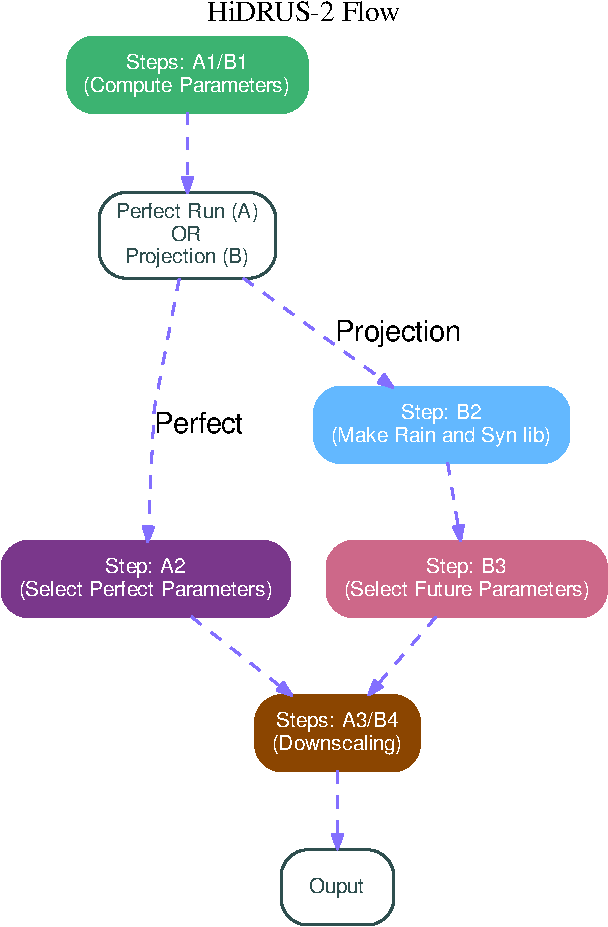
\includegraphics[width=6in]{./fig/flow.pdf}

\subsection{Compute Cascade Parameters}
\begin{lstlisting}[style=BashInputStyle]
	$ cd ~/data/mel-radar/
	$ /Path/to/mkCascParm_dbz ./ 02
\end{lstlisting}
 After program finish 
 
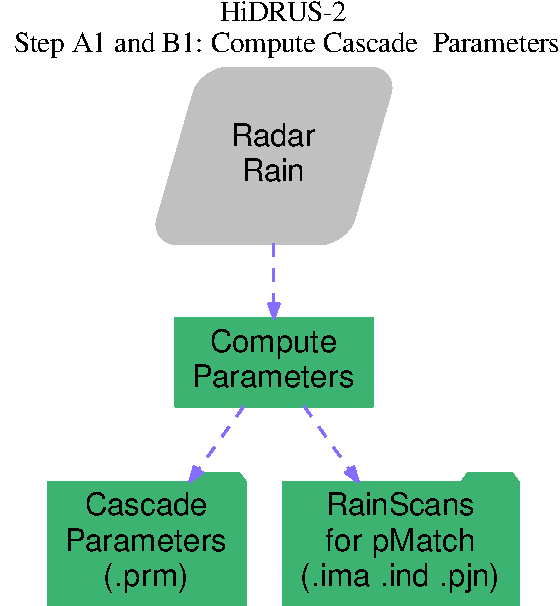
\includegraphics[width=4in]{./fig/casc_prm.pdf}
 
 
\begin{lstlisting}[style=BashInputStyle]
	$ cd ./c_params_dbz/
\end{lstlisting}

\subsection{Run With Perfect Parameters}
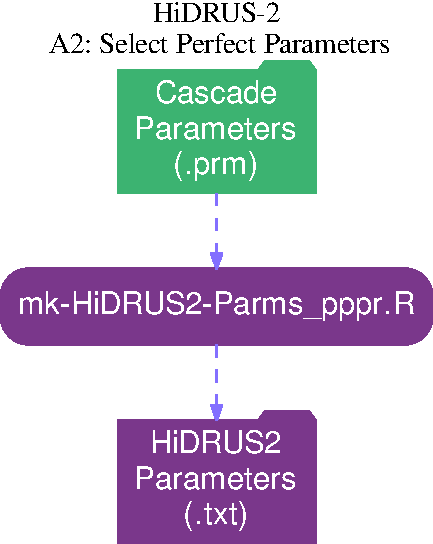
\includegraphics[width=4in]{./fig/perf_prm.pdf}\\
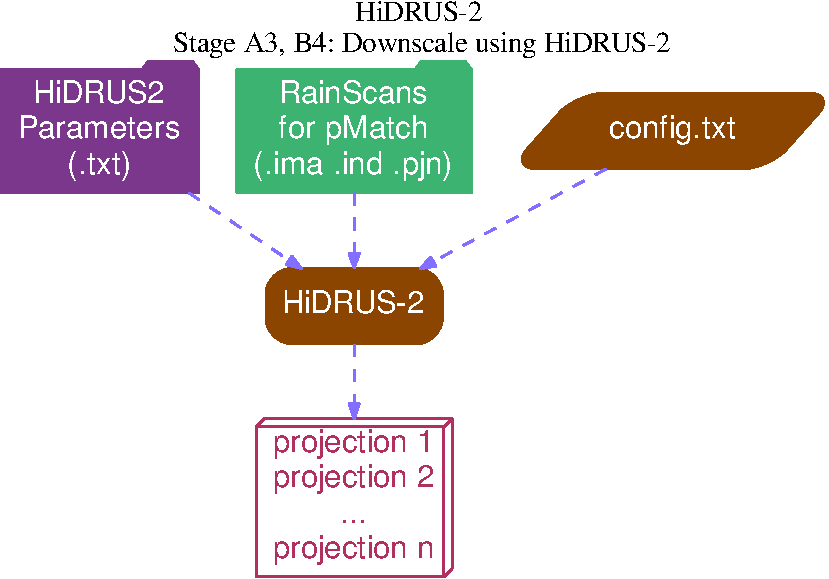
\includegraphics[width=4in]{./fig/runPerf_h2.pdf}

\subsection{Run for Prediction}

\subsubsection{Make Rain Library}
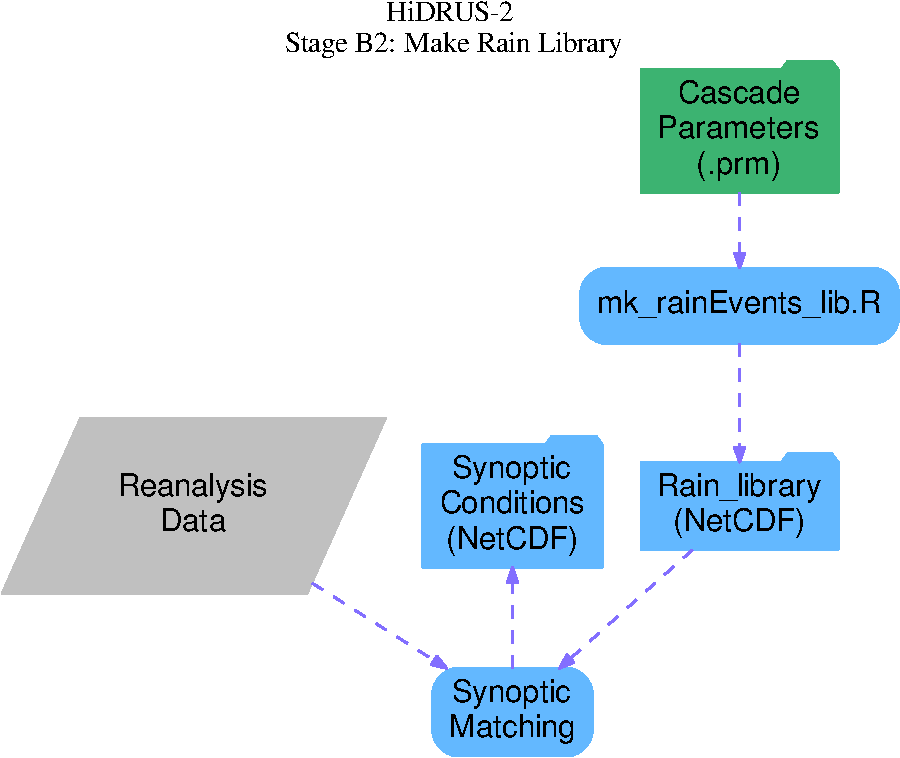
\includegraphics[width=4in]{./fig/mkRainlib.pdf}


\subsubsection{Add auxiliary data to the Rain Library}

\subsubsection{Select Future Parameters}
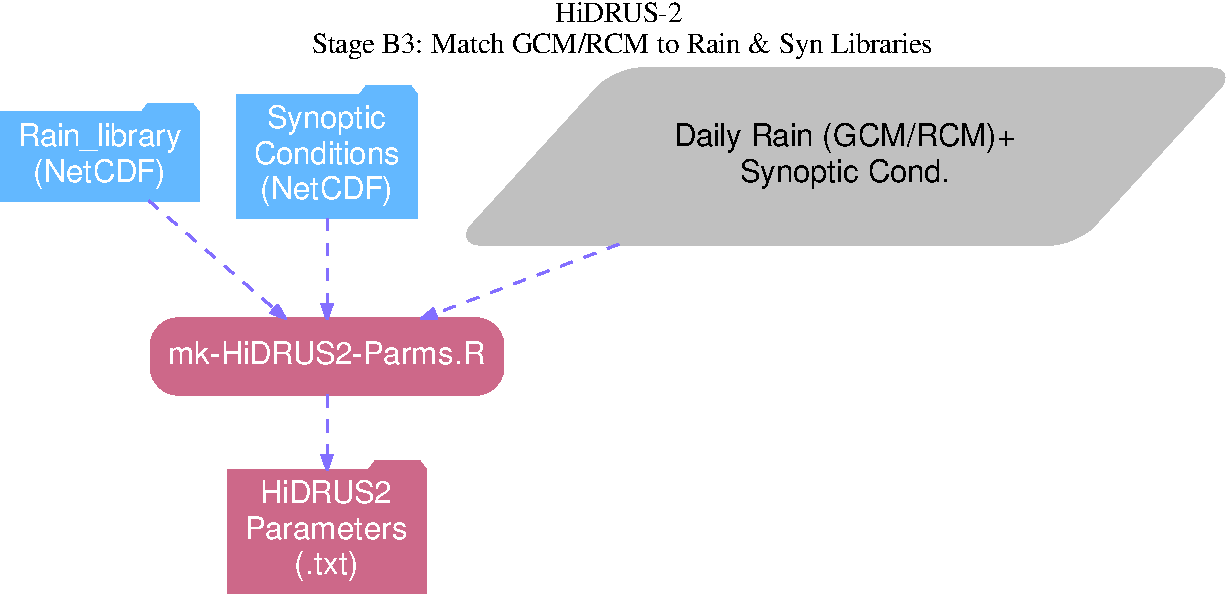
\includegraphics[width=6in]{./fig/selFuturePrm.pdf}


\subsubsection{Run HiDRUS-2}
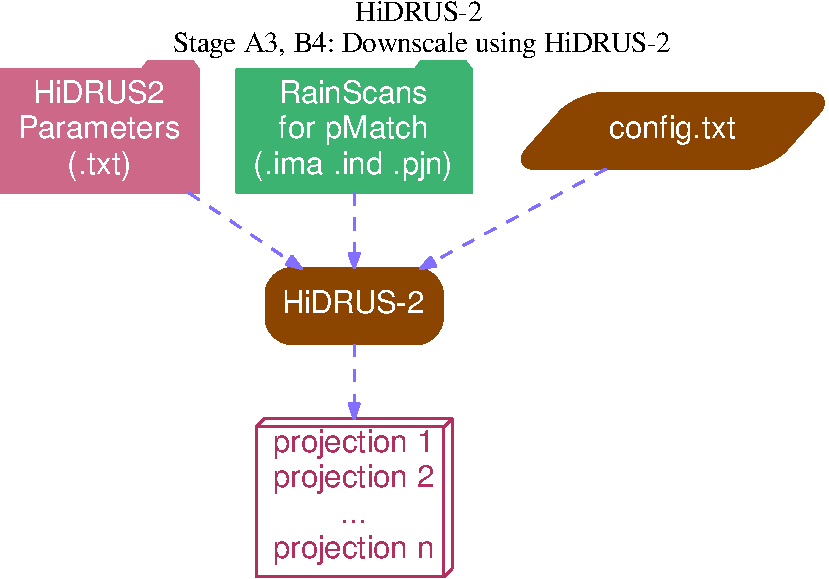
\includegraphics[width=6in]{./fig/runH2.pdf}

\subsection{Selecting Parameters}
First make a file with field mean rainfall (for the domain) from the GCM/RCM rainfall. 
I use CDO to crop and take field mean as follows.

\begin{lstlisting}[style=BashInputStyle]
	$ cdo fldmean -sellonlatbox,143.5,146,-36.5,-39 
	  Rain_dailyAccum.nc Rain_dailyAccum_fmean_MLB.nc
\end{lstlisting}

mk-HiDRUS2-Parms.R is an example of paramter selection for the HiDRUS-2 model. This script takes in the daily rainfall file, rainfall library files produced in the preprocessing stage and produces a large ASCII file to run the HiDRUS model. This script selects the most suitable event for the future rainy day and assigns all the parameters of that day to the corresponding future day.
HiDRUS-2 may/may not not use all the parameters in the file.


\bibliographystyle{IEEEtranN}
\bibliography{references}


\end{document}